\chapter{Porównanie architektury} \label{chap:porownanie}
Choć porównywanie kombinacji bibliotek z językiem programowania wydaje się dziwne, to jeżeli spojrzy się na funkcjonalności oferowane przez Reacta i Reduxa w porównaniu do możliwości Elma, można zauważyć pewne podobieństwa w sposobie budowania aplikacji. W tym rozdziale zostały opisane funkcjonalności, które są oferowane przez oba rozwiązania, oraz różnice występujące między Reactem i~Reduxem a Elmem dla każdej z funkcjonalności.

\section{Virtual DOM i składnia}
\subsection{Document Object Model}
DOM \footnote{z. ang. Document Object Model} jest niezależnym od platformy i języka programowania interfejsem, który pozwala programom i skryptom na dynamiczny dostęp i aktualizację treści, struktury i stylu dokumentu. Kiedy strona internetowa jest ładowana, przeglądarka tworzy DOM strony, będący obiektową reprezentacją dokumentu HTML. Służy ona jako interfejs umożliwiający pobieranie oraz modyfikację elementów HTML, które w DOM-ie są zdefiniowane jako obiekty.

\subsection{Dlaczego DOM jest powolny?}
Każda akcja na stronie powoduje zmianę DOM-u. Ze względu na jego drzewiastą strukturę, sama modyfikacja DOM-u jest szybka. Jednak każdy z modyfikowanych elementów oraz wszystkie jego dzieci muszą dodatkowo przejść przez dwa kosztowne etapy:
\begin{enumerate}
	\item Reflow będący procesem, podczas którego przeliczane zostają wymiary oraz pozycja elementu. Dokładnie ten sam proces jest uruchamiany na węzłach dzieci, a także elementach, które pojawiają się w DOM-ie później niż główny element. Reflow jest kosztowny, ponieważ zmiana pojedynczego elementu w strukturze DOM-u może spowodować wywołanie Reflow na wielu innych elementach.
	\item Repaint, w którym niektóre partie ekranu muszą zostać zaktualizowane, czy to ze względu na modyfikacje wymiarów i~pozycji elementu, czy przez zmiany stylistyczne, takie jak zmiana koloru tła. Etap ten jest kosztowny ponieważ przeglądarka musi sprawdzić widoczność innych węzłów w~DOM-ie.
\end{enumerate} 

\subsection{Virtual DOM}
Virtual DOM jest to lekka, niezależna od przeglądarki abstrakcyjna reprezentacja DOM-u. Służy ona między innymi do zminimalizowania kosztu stworzonego przez etapy Reflow i Repaint. Zamiast tworzyć za każdym razem drzewo składające się z węzłów DOM-u, Virtual DOM pozwala na stworzenie tego drzewa przy pomocy abstrakcyjnych węzłów, które są odpowiednikami faktycznych elementów DOM-u. Dzięki temu wszystkie operacje modyfikujące widok mogą być wykonane na abstrakcyjnej strukturze, a dopiero końcowy rezultat powoduje modyfikację faktycznego DOM-u.

\subsection{Algorytm porównywania różnic}
Koncepcja Virtual DOM-u została wykorzystana do tego, aby w każdej klatce budować zupełnie nową scenę. Choć taka operacja wydaje się kosztowna, to tak naprawdę zbudowanie pełnego drzewa Virtual DOM-u jest szybkie, i jest wykorzystywane przy każdej aktualizacji widoku. W momencie gdy następuje zmiana powodująca modyfikację widoku, algorytm porównuje ze sobą stare i nowe drzewo Virtual DOM-u. Wszystkie komponenty, w których nastąpiła jakakolwiek zmiana są oznaczane specjalną flagą, która określa, że dany węzeł został zmodyfikowany. Na tej podstawie budowana jest dokładna lista zmian jakie nastąpiły w widoku. Następnie lista ta jest wykorzystywana do modyfikacji faktycznego DOM-u, lecz nie jako pojedynczo wprowadzane zmiany, a jedna aktualizacja drzewa dokumentu. 

\begin{figure}[h]
	\centering
	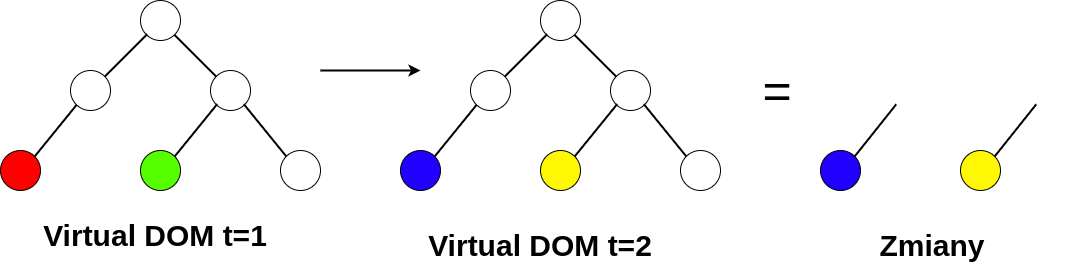
\includegraphics[width=0.8\textwidth]{images/diff_algorithm}
	\caption{Schemat działania algorytmu  porównywania różnic}
	\label{fig:diffAlgorithm}
\end{figure}

\subsection{Reprezentacja w Elmie}
Zarówno React, jak i Elm posiadają własne implementacje Virtual DOM-u. W Elmie abstrakcyjną reprezentację węzła otrzymujemy przy pomocy funkcji \lstinline{node}, która jako atrybuty przyjmuje tag, listą atrybutów HTML, oraz listę węzłów dzieci:
\begin{lstlisting}[style=elm-style]
	node : String -> List Attrbiute -> List Html -> Html
\end{lstlisting}
W przypadku użycia tagów HTML, takich jak \lstinline{div}, Elm udostępnia funkcje pomocnicze, które posiadają już uzupełniony atrybut tag, pozostawiając nam do określenia atrybuty węzła oraz jego dzieci. Elm nie ma specjalnej składni, która służyłaby do budowania widoków. Wszystkie elementy, z których budowany jest widok aplikacji, są funkcjami. W przypadku budowania widoku jedynym wymaganiem jest, aby funkcja go budująca zwracała rekord specjalnego typu \lstinline[style=elm-style]{Html msg}, który jest głównym blokiem służącym do tworzenia wyjściowego kodu HTML.

\subsection{Reprezentacja w React}
W przypadku Reacta mamy do czynienia ze znacznie bardziej rozszerzonym podejściem.  Bazowym elementem reprezentującym abstrakcyjny węzeł Virtual DOM-u jest ReactElement. Analogicznie jak w przypadku funkcji \lstinline{node} w Elmie jest to obiekt posiadający informację o tagu, który reprezentuje, atrybutach zdefiniowanego węzła, oraz listę dzieci. Przykład tworzenia takiego elementu można zobaczyć we fragmencie kodu \ref{listing:jsreactelement}. 

\begin{minipage}{.45\textwidth}
	\begin{lstlisting}[caption=Javascript,style=JavaScript,label = listing:jsreactelement]
	var divHello = React.createElement(
	"div",
	{ className: "myclass" },
	"Hello world!"
	);
	\end{lstlisting}
\end{minipage}\hfill
\begin{minipage}{.45\textwidth}
	\begin{lstlisting}[caption=JSX,style=JavaScript,firstnumber=1,label = listing:jsx]
	var divHello = (
	<div className="myclass">
		Hello world!
	</div>
	);
	\end{lstlisting}
\end{minipage}

\subsection{Test wydajnościowy}
Biorąc pod uwagę to, że każdy element Virtual DOM-u w React'cie jest zbudowany w podobny sposób, można zauważyć, że w przypadku rozbudowanej aplikacji, kod bardzo szybko staje się skomplikowany i niezrozumiały. Aby tego uniknąć, Facebook stworzył specjalne rozszerzenie składni dla JavaScriptu -- JSX. Z wyglądu przypomina składnię języka HTML, lecz zasadniczo dostarcza cukier syntaktyczny dla funkcji \lstinline[style=JavaScript]{createElement}. Fragmenty kodu \ref{listing:jsx} oraz \ref{listing:jsreactelement} są dokładnie tymi samymi wyrażeniami, z tą różnicą, że w drugim przypadku został wykorzystany JSX. Takie podejście pozwala na użycie JSX-a wewnątrz instrukcji JavaScriptu, przypisywanie go do zmiennych, czy też zwracanie z funkcji. Operacja zachodzi także w drugą stronę, co znaczy, że można korzystać z kodu JavaScriptu wewnątrz składni JSX-a. Taki kod musi być objęty nawiasami klamrowymi, aby odróżnić fragmenty napisane w JavaScript'cie od kodu JSX-a. 

% Test czasu renderowania
Choć główne założenia Virtual DOM-u w Elmie i React'cie są podobne, to jego implementacje nie są identyczne, w związku z czym można je porównać pod względem wydajnościowym. W tym przypadku wykorzystany został test wydajnościowy stworzony przez twórcę Elma \cite{perComp}. Pozwala on na porównanie czasu renderowania różnych implementacji aplikacji TodoMVC. Jest to prosty projekt listy zadań, umożliwiający dodawanie i usuwanie wpisów, oznaczanie ich jako zakończone, a także odfiltrowywanie na podstawie statusu wpisów. Test zakłada realistyczny scenariusz, w którym każda zmiana jest wyświetlona jako pojedyncza klatka, tak jakby to faktyczny użytkownik przeprowadzał test. Algorytm scenariusza wykonywany w trakcie pomiaru średniego czasu renderowania wygląda następująco:
\begin{enumerate}
	\item Stworzenie strony niezawierającej wpisów
	\item Dodanie 100 wpisów do listy
	\item Oznaczenie każdego z elementów jako zakończony
	\item Usunięcie wszystkich wpisów
\end{enumerate}
Dodatkowo zostały przyjęte następujące założenia, które sprawiają, że przeprowadzony test jest sprawiedliwy:
\begin{enumerate}
	\item Brak zgrupowanych zdarzeń -- oznacza to, że zamiast generować zdarzenia w pojedynczej pętli, algorytm tworzy jedno zdarzenie na raz, przechodząc do następnego dopiero po wyrenderowaniu całego widoku. Gdyby takie założenie nie zostało przyjęte, to przykładowo w przypadku dodawania wpisów, zmiany następowałyby na tyle szybko, że zamiast wyświetlić 100 klatek, przeglądarka wyświetliłaby tylko jedną.
	\item Brak użycia \lstinline{requestAnimationFrame} -- funkcja ta informuje przeglądarkę o zamiarze wykonania animacji i żąda od przeglądarki wywołania określonej funkcji w celu odświeżenia animacji przed następną zmianą w widoku. Oznacza to, że odświeżenie animacji jest wyrównane do 60 razy na sekundę, niezależnie od tego, jak wiele klatek wygeneruje JavaScript. Elm wykorzystuje tą funkcję do pomijania części klatek, które i tak nie będą widoczne dla użytkownika. W z związku z realistycznym scenariuszem, oraz brakiem podobnej optymalizacji w innych implementacjach, funkcja ta musiała zostać usunięta z Elma w ramach przeprowadzanego testu.
\end{enumerate}

\begin{figure}[h]
	\centering
	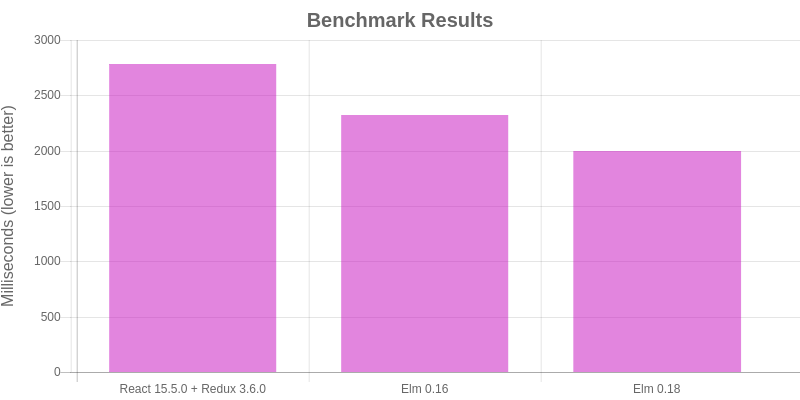
\includegraphics[width=0.9\textwidth]{images/render_comparision}
	\caption{Porównanie czasu renderowania aplikacji TodoMVC (w oparciu o \cite{perComp})}
	\label{fig:performanceComparision}
\end{figure}

Na rysunku \ref{fig:performanceComparision} można zauważyć, że zostały wzięte pod uwagę dwie wersje Elma. Powodem jest tutaj zmiana używanej implementacji Virtual DOM-u. Od początku istnienia Elma aż do wersji 0.16, wykorzystywana była implementacja Matta Escha, która była silnie inspirowana wersją Virtual DOM-u wykorzystywaną w React'cie. Jednak z powodu dużych zmian wprowadzonych w nowszych wersjach Elma, twórca języka był zmuszony stworzyć własną implementację dopasowaną do nowego API. 

Wyniki testu pokazują, że implementacja aplikacji w Elmie jest szybsza o ponad sekundę. Twórca Elma w jednym ze swoich artykułów \cite{blazingFastHtml} pisze o wykorzystanych technikach, które są powodem takich wyników:
\begin{enumerate}
	\item Używanie tablic zamiast słowników -- iteracja po tablicy jest zawsze o wiele szybsza operacją niż przechodzenie po kluczach słownika.
	\item Minimalizacja ilości alokacji -- garbage collection jest jednym z kosztownych elementów w analizowanych implementacjach. Im mniej obiektów jest alokowanych, tym lepsza jest wydajność aplikacji. Sposób wykorzystany w Elmie polega na alokowaniu obiektów z pustymi polami. Dzięki temu silniki JavaScriptowe radzą sobie o wiele lepiej z optymalizacją takich obiektów, a obiekt nie zmienia się, nawet gdy wypełnimy go większą ilością informacji.
	\item Unikanie powolnych operacji, takich jak pobieranie konkretnego elementu z tablicy. 
\end{enumerate}

\section{Jednokierunkowy przepływ danych}
\subsection{Architektura języka Elm}
Jednokierunkowy przepływ danych w języku Elm jest często określany jako \textit{Architektura języka Elm} lub \textit{Model-View-Update}. Niezależnie od rozmiaru tworzonej aplikacji, każdą z nich można podzielić na trzy całkowicie oddzielone od siebie części:
\begin{itemize}
	\item Model -- jest strukturą danych zawierającą wszystkie informacje o stanie aplikacji. W programie jest reprezentowany jako rekord o ściśle określonym typie.
	\item Update -- sposób, w jaki stan aplikacji jest aktualizowany, reprezentowany przez funkcję przyjmującą jako argumenty komunikat o rodzaju aktualizacji danych oraz dotychczasowy stan aplikacji, a zwracającą nowy, zaktualizowany stan.
	\item View -- definicja sposobu wyświetlania stanu aplikacji w formie kodu HTML. Jest reprezentowany przez funkcję przyjmującą jako argument aktualny stan aplikacji, a zwracającą reprezentację kodu HTML w formie obiektów Virtual DOM-u.
\end{itemize}
\begin{figure}[h]
	\centering
	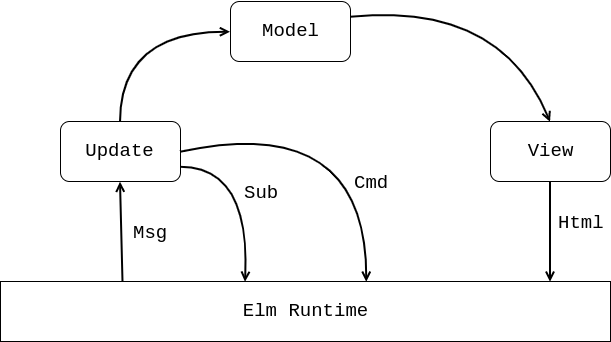
\includegraphics[width=0.6\textwidth]{images/elm_data_flow}
	\caption{Przepływ danych w języku Elm}
	\label{fig:elmFlow}
\end{figure}
\FloatBarrier
Niezależnie od rodzaju wykonywanej akcji, przepływ danych w języku Elm opiera się o podstawowe struktury zwane wiadomościami. Są to komunikaty zdefiniowane przez programistę w kodzie, które poza typem wiadomości mogą zawierać dane, na podstawie których aktualizowany jest modek. Silnik języka przesyła je wraz z aktualną wersją modelu do funkcji \lstinline{update}, która na podstawie rodzaju wiadomości oraz zawartych w niej danych aktualizuje model. Nowa wersja modelu zostaje następnie przekazana do funkcji \lstinline{view}, która buduje na jego podstawie pełną strukturę opisującą widok. Struktura ta, będąca obiektem typu \lstinline[style=elm-style]{Html}, skonstruowanym przy pomocy funkcji z implementacji Virtual DOM-u, jest następnie przesyłana do silnika Elma, który na jej podstawie aktualizuje drzewo DOM-u.

Elm posiada także dwa dodatkowe rodzaje komunikatów: komendy i subksrypcje. Te pierwsze odpowiadają za wysyłanie wiadomości obsługujących efekty uboczne, takie jak zapytania HTTP. Są one tworzone jako obiekty typu \lstinline[style=elm-style]{Cmd} posiadające w sobie typ wiadomości, jaka ma zostać wywołana. Obiekty takie są wysyłane równocześnie z modelem, jako część zwrotna funkcji \lstinline{update}, która wysyła model do funkcji odpowiadającej za budowę widoku, natomiast samą komendę przekazuje do silnika Elma. Silnik na podstawie podanej komendy wywołuje kolejną aktualizację modelu, jako wiadomość przekazując zawartość komendy. Subskrypcje natomiast, są sposobem na nasłuchiwanie zewnętrznych komunikatów takich jak ruchy myszy, zmiana adresu w przeglądarce, czy też zmiana jej rozmiaru. Są one zdefiniowane podczas uruchomienia aplikacji jako obiekty typu \lstinline[style=elm-style]{Sub}, które podobnie jak w przypadku komend posiadają w sobie typ wiadomości, która po nastąpieniu zewnętrznego zdarzenia jest wysyłana przez silnik języka do funkcji \lstinline{update}.

Prostota tak skonstruowanego przepływu danych pozwala na łatwą analizę działania aplikacji, niezależnie od jej rozmiaru. Programista nie jest zmuszony do zastanawiania się nad skomplikowaną architekturą, dzięki czemu jest w stanie szybko ustalić, w jaki sposób działa aplikacja. Prosty model aktualizacji danych oparty na komunikatach pozwala także na łatwe dodawanie nowych funkcjonalności, ponieważ wiąże się to z dodaniem nowego komunikatu, który jest definiowany niezależnie od poprzednio dodanych wiadomości.

\subsection{Komponent prezentacyjny i kontener}
Aby w ogóle zacząć temat jednokierunkowego przepływu danych w kombinacji React i Redux, trzeba wyjaśnić, czym są komponenty. W przeciwieństwie do Elma, który całą swoją strukturę opiera na funkcjach, React wprowadza specjalny rodzaj struktur umożliwiający zdefiniowanie wyświetlanych widoków.

W dokumentacji Reacta można znaleźć, że komponenty pozwalają podzielić interfejs na niezależne fragmenty wielokrotnego użytku i myśleć o każdym z fragmentów oddzielnie \cite{reactDocs}. Koncepcyjnie są one podobne do funkcji w JavaScript'cie. Przyjmują dowolne dane wejściowe, które zawarte są w pojedynczym obiekcie \lstinline{props}, a zwracają elementy Reacta, opisujące to, co powinno zostać wyświetlone. Fragmenty \ref{listing:statelesscomp} i \ref{listing:statefulcomp} przedstawiają dwa podstawowe sposoby tworzenia komponentów w React'cie: jako zwykła funkcja JavaScript oraz jako klasa ze standardu ECMAScript 6.
\newpage % Simple hack to remove first line of listing from page end
\begin{lstlisting}[style=JavaScript, caption=Funkcyjny komponent bezstanowy, label=listing:statelesscomp]
function Welcome(props) {
	return <h1>Hello, {props.name}</h1>;
}
\end{lstlisting}

\begin{lstlisting}[style=JavaScript, caption=Komponent stanowy jako klasa ECMAScript 6, label=listing:statefulcomp]
class Clock extends React.Component {
	constructor(props) {
		super(props);
		this.state = {date: new Date()};
	}
	render() {
		return (
			<div>
				<h1>It is {this.state.date.toLocaleTimeString()}.</h1>
			</div>
		);
	}
}
\end{lstlisting}
W pierwszym przypadku mamy do czynienia z komponentem funkcyjnym bezstanowym. Zgodnie z~jego nazwą charakteryzuje się brakiem lokalnego stanu oraz zapisem w formie funkcji przyjmującej jako argument obiekt \lstinline{props}, która zwraca elementy Reacta. Komponent tego typu nie pozwala także na zarządzanie jego cyklem życia, czy optymalizacją częstotliwości odświeżania. Aby skorzystać z tych funkcjonalności, należy użyć implementacji za pomocą klasy. Komponenty klasowe umożliwiają dodanie logiki do cyklu życia komponentu, co sprawia, że stają się one czymś więcej niż tylko obiektami opisującymi jakie elementy mają zostać wyświetlone na interfejsie użytkownika.

W kontekście połączenia Reacta i Reduxa często stosuje się inny podział, na komponenty prezentacyjne i kontenery. Różnią się one od siebie przede wszystkim tym, że kontenery są specjalnym rodzajem komponentów, które są świadome istnienia Reduxa. To one odpowiadają między innymi za pobranie danych ze stanu Reduxa, czy wysyłaniu akcji określających, w jaki sposób ma zostać zmieniony stan. Pobieranie danych w kontenerze się to poprzez użycie funkcji \lstinline{connect} ze specjalnej biblioteki \textit{react-redux} zawierającej kod wymagany do współpracy Reacta z Reduxem \cite{reduxDocs}. Funkcja \lstinline{connect} przyjmuje jako argument zdefiniowaną przez użytkownika funkcję określającą, który fragment stanu Reduxa ma zostać użyty w kontenerze. W przypadku komponentów prezentacyjnych jedynym źródłem danych są właściwości przekazane za pomocą obiektu \lstinline{props}, a jedynym możliwym sposobem na zmianę stanu są funkcje zwrotne, również przekazane jako część tego obiektu.

Powodem takiego podziału jest przede wszystkim oddzielenie komponentów widoku, które mogą być używane wielokrotnie i nie powinny zależeć od implementacji logiki odpowiadającej za pobieranie i zarządzanie danymi.

\subsection{Przepływ danych w Redux i lokalny stan komponentów}
Twórca Reduxa tworząc implementację biblioteki, inspirował się między innymi Elmem, w związku z~czym sposób przepływu danych występujący w bibliotece Redux jest bardzo zbliżony do implementacji z języka Elm, a pewne fragmenty Reduxa można porównać do części architektury \textit{Model-Update-View}.

Odpowiednikiem modelu jest pojedyncze drzewo stanu zawierające w sobie wszystkie dane aplikacji. Różnica występująca między implementacją w Elmie jest brak ograniczenia co do typu, co pozwala na dowolną modyfikację drzewa, bez zbędnej potrzeby wcześniejszego definiowania domyślnych wartości. 

Tak jak w Elmie podstawową strukturą służącą do komunikowania o aktualizacji jest wiadomość, tak w przypadku Reduxa wykorzystywane są akcje. Są to zwykłe obiekty JavaScriptu posiadające informacje o rodzaju komunikatu, a także mogące posiadać dane wykorzystane do aktualizacji. W przeciwieństwie do Elma Redux nie posiada dodatkowych komunikatów służących do obsługi efektów ubocznych czy zdarzeń z zewnątrz, co zmusza programistę do skorzystania z innych bibliotek obsługujących takie zdarzenia. Przykładem tutaj może być biblioteka \textit{redux-saga}, służąca do obsługi efektów ubocznych \cite{reduxSaga}, która dodatkowo wspiera komunikację z Reduxem.

\begin{figure}[h]
	\centering
	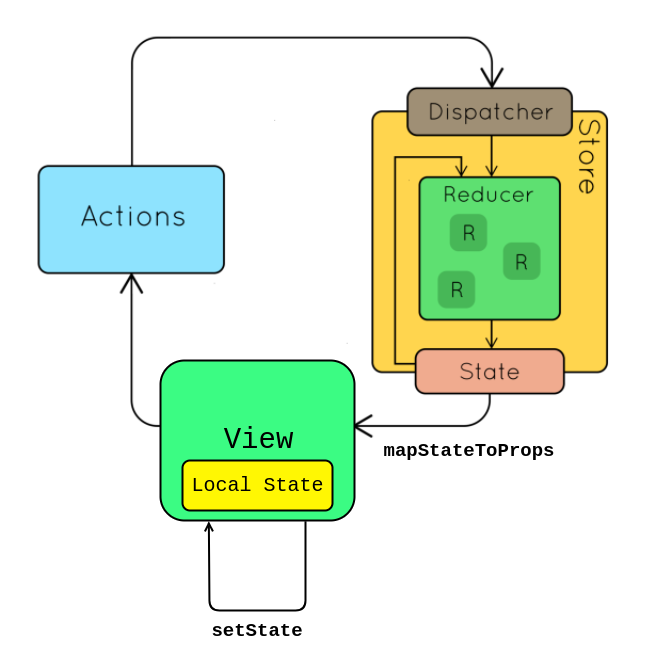
\includegraphics[height=0.37\textheight]{images/react_redux_data_flow}
	\caption{Przepływ danych w kombinacji React i Redux}
	\label{fig:reactReduxFlow}
\end{figure}
\FloatBarrier


Aktualizacja danych odbywa się za pomocą funkcji zwanych \textit{reducer'ami}. Są to funkcje bez efektów ubocznych, które na podstawie dotychczasowego stanu oraz akcji zwracają nowe, zaktualizowane drzewo stanu. W przypadku Reduxa programista nie jest zmuszony do tworzenia jednej funkcji odpowiadającej za wszystkie aktualizacje. Biblioteka udostępnia funkcję \lstinline{combineReducers}, przyjmującą wszystkie funkcje, które mają posłużyć jako reducer. Po przysłaniu akcji uruchamiane są wszystkie przekazane wcześniej funkcje, a wyniki z każdej z nich są wstawiane do jednego obiektu głównego, który reprezentuje całość stanu aplikacji.

W kombinacji Reacta i Reduxa za warstwę widoku odpowiadają komponenty, które, tak jak zostało to wcześniej opisane, można podzielić na kontenery i komponenty prezentacyjne. Jednak w przeciwieństwie do sposobu budowania widoku w Elmie, opartego na pojedynczej funkcji przyjmującej cały model aplikacji, to kontenery decydują o tym jakie informacje chcą pobrać z drzewa stanu. Odbywa się to przy pomocy specjalnie zdefiniowanej przez programistę funkcji \lstinline{mapStateToProps}, jako argument przyjmującej stan aplikacji, a zwracającą tylko oczekiwany przez kontener fragment danych. 

To, co zaburza w pewien sposób jednokierunkowość przepływu danych oferowaną przez Reduxa, to lokalny stan komponentów. Zarówno komponenty prezentacyjne, jak i kontenery mają możliwość posiadania własnego stanu, przypisanego do konkretnej instancji komponentu. Stan taki jest całkowicie niezależny od drzewa stanu z Reduxa. Każda jego zmiana, odbywająca się poprzez funkcję \lstinline{setState}, przyjmującą jako argument nowy stan, powoduje odświeżenie widoku. Lokalny stan sprawia, że nie posiadamy już jednego źródła danych, co może doprowadzić do ich potencjalnej duplikacji. Z drugiej strony jednak, lokalny stan jest zwykle wykorzystywany do zarządzania opcjami widoku, które nie powinny być częścią źródła danych jakim jest drzewo stanów z Reduxa. Gdyby doszło do takiej sytuacji, to na każdą nową instancję komponentu przypadałby jeden nowy obiekt określający opcje widoku tego komponentu. Powodowałoby to szybki i niepotrzebny rozrost drzewa stanu.

\section{Niemutowalność obiektów i ograniczenia typów}
Ważnymi elementami architektury, które Elm udostępnia domyślnie, jest niemutowalność obiektów oraz silne typowanie. Obie te funkcjonalności znacząco wpływają na sposób modelowania danych już od samego początku tworzenia aplikacji. 

\subsection{Silne typowanie w Elmie, a ograniczenia typów w React i Redux}
Programista, tworząc model stanu aplikacji, jest zmuszony do określenia typu dla każdego z elementów. Także każda implementacja funkcji posiada z góry określone typy przyjmowanych argumentów oraz typ zwracanej struktury. Dzięki temu wszelkie niezgodności typów mogą zostać wykryte już na poziomie kompilacji kodu, niezależnie od tego, jak mocno zagłębiona jest różnica. Pozwala to na uniknięcie wystąpienia wyjątków w trakcie działania aplikacji. W przypadku kombinacji Reacta i Reduxa ograniczenie typów można uzyskać poprzez wykorzystanie rozszerzeń języka JavaScript, takie jak TypeScript. Dodatkowo React posiada wbudowane sprawdzanie typów w kontekście komponentów. Każdy z komponentów może posiadać zdefiniowane przez użytkownika właściwości, których typy można określić za pomocą dodatkowej opcji \lstinline{propTypes}. Dla każdej z właściwości można określić jeden z następujących typów:
\begin{itemize}
	\item Typy prymitywne JavaScriptu: typ logiczny, funkcja, liczba, obiekt, łańcuch znaków, symbol
	\item Element Reacta -- mogą być to komponenty lub podstawowe elementy z języka HTML
	\item Wieloelementowa struktura danych -- możemy określić jakiego typu są poszczególne elementy struktury
	\item Typy niestandardowe -- zamiast typu podawana jest funkcja, która pozwala przeprowadzić walidację podanego obiektu pod względem zawartości czy nawet nazewnictwa
	\item Typ dowolny -- właściwość określona tym typem nie posiada żadnych ograniczeń co do zawartości
	\item Jeden z wielu -- jest to ograniczenie zarówno co do typu, jak i co do zawartości. Programista może zdefiniować do jakich konkretnych wartości, czy typów może ograniczać się podana właściwość
\end{itemize}
Typ zawiera także informację o tym czy dany element jest wymagany.

\subsection{Niemutowalność obiektów}
Niemutowalność obiektów zarówno w przypadku tworzenia aplikacji w języku Elm, jak i przy pomocy kombinacji Reacta i Reduxa, jest bardzo istotna ze względu na możliwości, które można zebrać w~trzech kategoriach: wydajność, przewidywalność oraz obserwowanie zmian. 

Wprowadzenie modyfikacji do niemutowalnego obiektu oznacza, że należy utworzyć jego nową instancję, co może wydawać się kosztowną operacją, ponieważ w teorii wszystkie wartości muszą zostać skopiowane do nowego obiektu. Tak naprawdę, obiekty niemutowalne wykorzystują dzielenie struktur pomiędzy instancjami obiektu, co pozwala na znaczne zmniejszenie narzutu pamięci.
\begin{figure}[h]
	\centering
	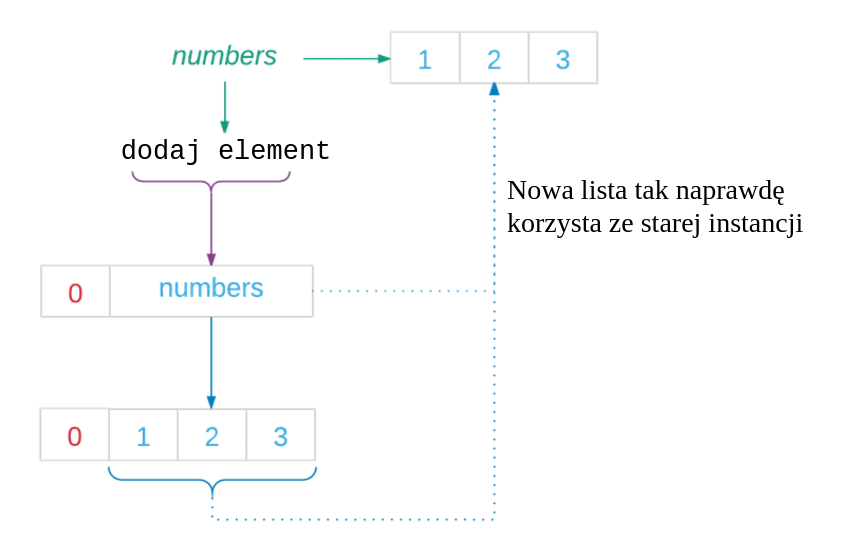
\includegraphics[width=0.5\textwidth]{images/structure_sharing}
	\caption{Dzielenie struktur w obiektach niemutowalnych}
	\label{fig:structSharing}
\end{figure}
Przykład, który obrazuje w jaki sposób działa dzielenie struktur w obiektach niemutowalnych można zobaczyć na rysunku \ref{fig:structSharing}. Dodanie elementu na początek listy tworzy nową instancję obiektu, jednak tak naprawdę część zawierająca elementy starej listy korzysta dokładnie ze struktury, która tworzyła starą instancję.

Użycie obiektów niemutowalnych do stworzenia stanu aplikacji zapobiega przed nieoczekiwaną zmianą stanu. Gdyby stan był zbudowany z mutowalnych obiektów, to po pobraniu go do części aplikacji odpowiadających za widok, mogłoby dojść do nieoczekiwanej modyfikacji stanu. O ile w Elmie taka sytuacja jest niemożliwa z powodu domyślnego występowania obiektów niemutowalnych, o tyle w~przypadku połączenia Reacta i Reduxa takie połączenie jest możliwe. Pomimo tego, że dokumentacja Reduxa zawiera całą sekcję na temat użycia obiektów niemutowalnych, to niestety nie jest to domyślna funkcjonalność. Gdy komponent Reacta pobiera dane z drzewa stanu i wywoływana jest funkcja \lstinline{render} definiująca widok, to użytkownik może chcieć odfiltrować część niepotrzebnych danych. Aby nie tworzyć kolejnej zmiennej, przypisze odfiltrowane wartości do zmiennej zawierającej dane pobrane bezpośrednio ze stanu. W przypadku użycia obiektów mutowalnych wartości zawarte w stanie zostaną nadpisane, a zmiana nie będzie w żaden sposób widoczna z poziomu Reduxa.

Śledzenie zmian obiektów niemutowalnych jest ważnym aspektem związanym z optymalizacją odświeżania widoku aplikacji. Zarówno Elm, jak i React udostępniają funkcje, które pozwalają określić, czy dany fragment widoku powinien zostać odświeżony. 

W przypadku Elma jest to funkcja \lstinline{lazy}, która przyjmuje jako argumenty funkcję implementującą dany fragmentu widoku oraz opcje, które służą jako argumenty do tejże funkcji. \lstinline{lazy} przed wywołaniem funkcji budującej konfigurację widoku porównuje czy przekazane argumenty są w jakikolwiek sposób zmodyfikowne w stosunku do ich poprzednich wartości. Domyślna niemutowalnosć obiektów w Elmie pozwala na to, aby funkcja ta tak naprawdę porównywała wyłącznie referencje obiektów.

Inaczej wygląda sytuacja w przypadku kombinacji Reacta i Reduxa. Każdy z komponentów może mieć zdefiniowaną funkcję \lstinline{shouldComponentUpdate} przyjmującą jako argumenty nowe wartości właściwości oraz lokalnego stanu. Jest ona uruchamiana przed odświeżeniem widoku i pozwala na ustalenie na podstawie nowych i starych wartości obiektów czy dany komponent powinien zostać odświeżony. Dodatkowo w przypadku kontenerów Redux dodaje automatyczne sprawdzenie wartości pobieranych z drzewa stanu, jednak nie są one porównywane w głąb. Programista zostaje więc zmuszony do zaimplementowania porównania w funkcji \lstinline{shouldComponentUpdate} w ten sposób, aby porównać wszystkie pola. Wprowadzenie niemutowalności obiektów rozwiązuje ten problem i sprawia, że porównanie zarówno właściwości, jak i lokalnego stanu komponentów sprowadza się, tak jak w Elmie, do porównania referencji obiektów, co znacznie zmniejsza koszt narzucany przez porównanie tych wartości przy każdym potencjalnym odświeżeniu komponentu.

Jednym z rozwiązań umożliwiających użycie obiektów niemutowalnych jest proponowana przez dokumentację Reduxa biblioteka Immutable.js \cite{reduxDocs}. Udostępnia ona niemutowalne struktury, takie jak lista, stos, mapa, zbiór czy rekord. Pozwala także na konwersję zwykłych obiektów JavaScriptu na struktury niemutowalne udostępniane przez bibliotekę, a także konwersje w drugą stronę. Niestety biblioteka ta ma też wady, które zwiększają przede wszystkim wymagany nakład czasu poświęconego na modelowanie danych. Jednym z głównych problemów jest to, że jeżeli użytkownik chce w pełni skorzystać ze wzrostu wydajności, jaki oferuje biblioteka w kontekście porównywania obiektów, jest on zmuszony do zarządzania tym, aby każdy element w strukturze danych był obiektem z biblioteki Immutable.js. Powodem jest to, że biblioteka przy wykonaniu konwersji na zwykły obiekt JavaScriptu tworzy za każdym razem nową instancję tego obiektu. W przypadku pobrania nowej i starej wersji obiektu, w którym nie nastąpiły żadne zmiany, próba porównania za pomocą referencji zakończy się niepowodzeniem, nawet jeśli wartości pól wewnątrz obu obiektów są dokładnie takie same.

